\section{Data Acquisition System}
 The data-acquisition (DAQ) system in Hall-A is composed of the CEBAF online data acquisition system (CODA) developed by the JLab CODA group, and the associated hardware components. CODA is a tool-kit of software components, including read-out controllers (ROCs), the event builder (EB), the event recorder (ER) and the event-transfer (ET). The other major component is the Run-Control (RC) which is a graphical user interface to choose experimental configurations, start and stop runs, and monitor and reset CODA components~\cite{halla_nim}. The hardware elements are basically composed of front-end Fastbus crates, VME devices (ADCs, TDCs and scalers), VME-Fastbus interfaces, single-board VME computers, trigger supervisors (TS) and network components. CODA is operated on a Linux based workstation which stores the recorded data (called raw data) in the local hard-drive. The data is subsequently transferred to a mass storage tape silo (MSS) for long term storage. Data in the local hard-drive will be deleted when the hard-drive runs out of space. 
 
  The E08-014 ran consecutively with four other experiments during the spring of 2011. Besides the HRSs, the BigBite spectrometer and a neutron detector were installed in the hall for double-coincidence and triple-coincidence experiments. Triggers from four devices were sent to the same TS located in the electronic hut on the floor. When a trigger was accepted by the TS, a Level-One-Accept (L1A) signal was generated and sent back to each spectrometer. The leading-edge of the L1A signal was then adjusted by the strobe signal in a retiming-module (RT) installed in the local front-end crate. The signal from RT was fed to the Transition Module (TM)~\cite{ts_tm}, where an ADC gate, a TDC Start/Stop signal and control signals were generated and distributed to the front-end electronics on Fastbus crates and VME crates where ADCs, TDCs and scalers start to record data when these signals arrive. An event number associated with this trigger was registered in the DAQ system and all signals associated with this events were recorded.
  
   Limited by the dead-time and data size, not all triggers were accepted by the TS. A pre-scale factor was assigned to each trigger type to control the total event rate before CODA starts taking data. For example, a pre-scale factor "3" represents the case that only the first one can be accepted for every three consecutive events from the trigger, and a pre-scale factor "0" means that no event from the trigger will be recorded. Each time when CODA starts to take data, a unique run number is given to the raw data file which stores all events coming after the start of the run. To control the total size of the data file and to prevent the data file from being damaged by any errors during the data taking, CODA will be stopped when each run reaches a pre-defined length of time or a certain number of events, and then a new run will be started with a new run number. 

   Scaler events are read every 1-4 seconds and stored in the data stream. Meanwhile, data from the Experimental Physics and Industrial Control System (EPICS), such as the beam energy, the BPM and BCM readings, the information of the target system, the angles and magnet fields spectrometers, etc., are also inserted into the data stream for every few seconds.

\section{Trigger Design}
  During the E08-014 the scattered electrons were measured by both HRSs simultaneously. The BigBite and the neutron detector were turned off and their triggers were ignored. Both HRSs shared the similar design of the trigger system which is illustrated in Fig.~\ref{trigger_design}. Three detector planes, S1, S2m and GC were included in the trigger design. A logic signal was created when one or more scintillator bar in S1 or S2m was fired. The logic signal of the GC was the digital signal converted from the sum of ten PMT signals. The coincidence of logic signals from S1, S2m and GC created T1 (T3) trigger in HRS-R (HRS-L), which was the production trigger in this experiment. T2 (T4) was formed in HRS-R (HRS-L) by the coincident signal of the GC logic signal and only one of the S1 or S2m logic signal. T2 (T4) was designed to evaluate the trigger efficiency of T1 (T3). T6 (T7) was generated from the overlapped signal of S1 and S2m, and is the traditional HRS main trigger. Events from T6 and T7 were used for particle identification study since pions were also recorded. T5 is the coincident signal of T1 and T3, and was disabled in this experiment. A discussion of triggers during the data analysis is given in Appendix A.
  
\begin{figure}[!ht]
 \begin{center}
  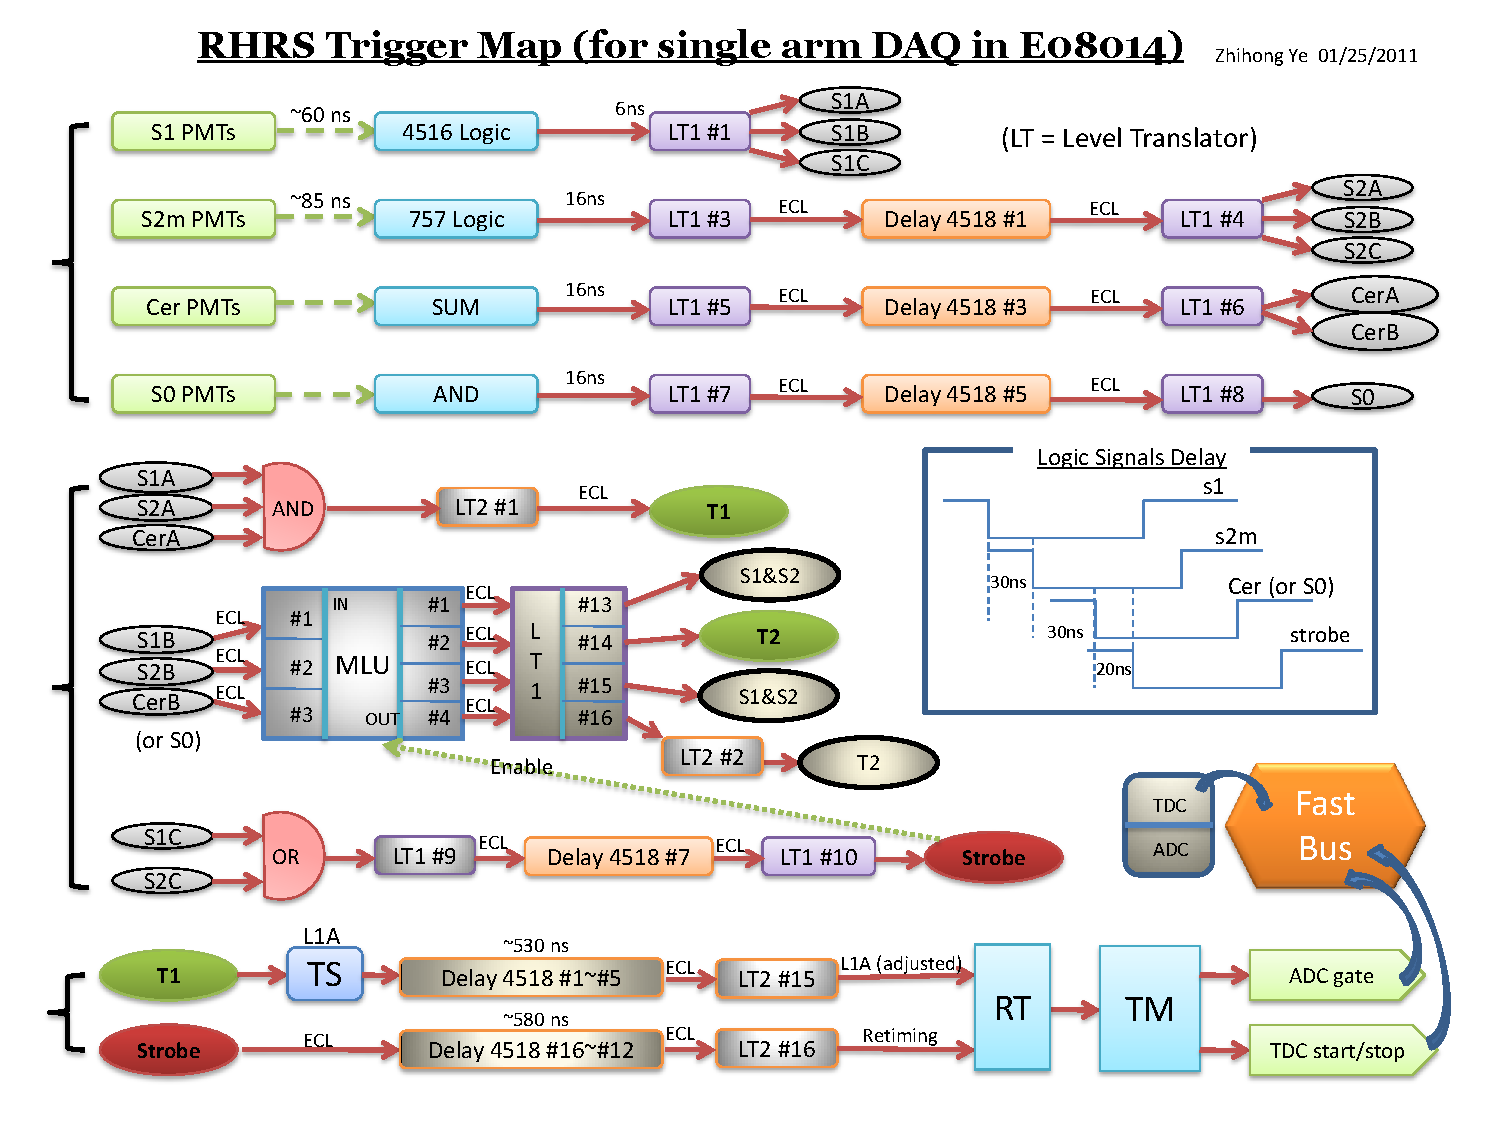
\includegraphics[angle=90,width=0.95\textwidth]{./figures/trigger/trigger_design}
  \caption[Single arm trigger design]{\footnotesize{Single arm trigger design on HRS-R, where the logic signal from the GC was also included to form the TS1 signal which produces the T1 trigger. The HRS-L trigger has the similar layout except some electronic modules were different.}}
  \label{trigger_design}
 \end{center}
\end{figure}
